\documentclass[tikz,border=10pt]{standalone}
\begin{document}
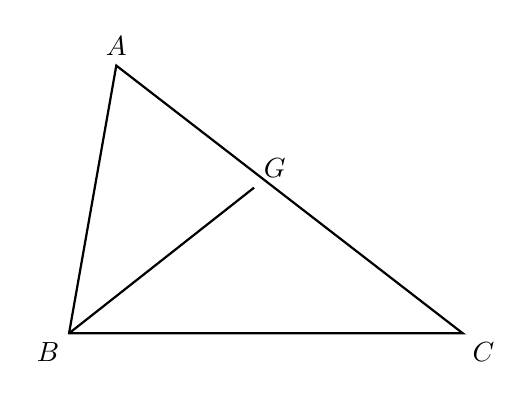
\begin{tikzpicture}
  \coordinate (A) at (0.6,3.4);
  \coordinate (B) at (0,0);
  \coordinate (C) at (5,0);
  \coordinate (G) at (2.35,1.85);

  \draw[thick] (A) -- (B) -- (C) -- cycle;
  \draw[thick] (B) -- (G);

  \node[above] at (A) {$A$};
  \node[below left] at (B) {$B$};
  \node[below right] at (C) {$C$};
  \node[above right] at (G) {$G$};
\end{tikzpicture}
\end{document}
